\chapter{Introduction}
\label{chap:introduction}
%Channel limit
%
%URC
%Deep fade
%drop out
%5G





For all types of communication an important aspect is the channel through which the message is transmitted. For wireless communication this is especially the case, as the channel changes constantly. The transmission of the message can be done in different environments, which have different impacts on the received signal. Common for nearly all the environments is that they introduce fading, which if not accounted for can have devastating effects on the transmission. 

Fading occurs when multipath propagation is present, that will introduce combinations of wavefronts that will add together either constructively or destructively as seen on \autoref{intro_fading}. The constructive areas is not of interest in this project, but instead the destructive interference which might result in outages are investigated. These spots are called deep fades or very deep fades and is where the communication might suffer an outage. An outage occurs if the transmitted signal drops below the receivers sensitivity level meaning the signal is lost. There are different tools to increase the chance to receive signals that might experience deep fades and therefore increase the reliability of the communication link


\begin{figure}[H]
\centering
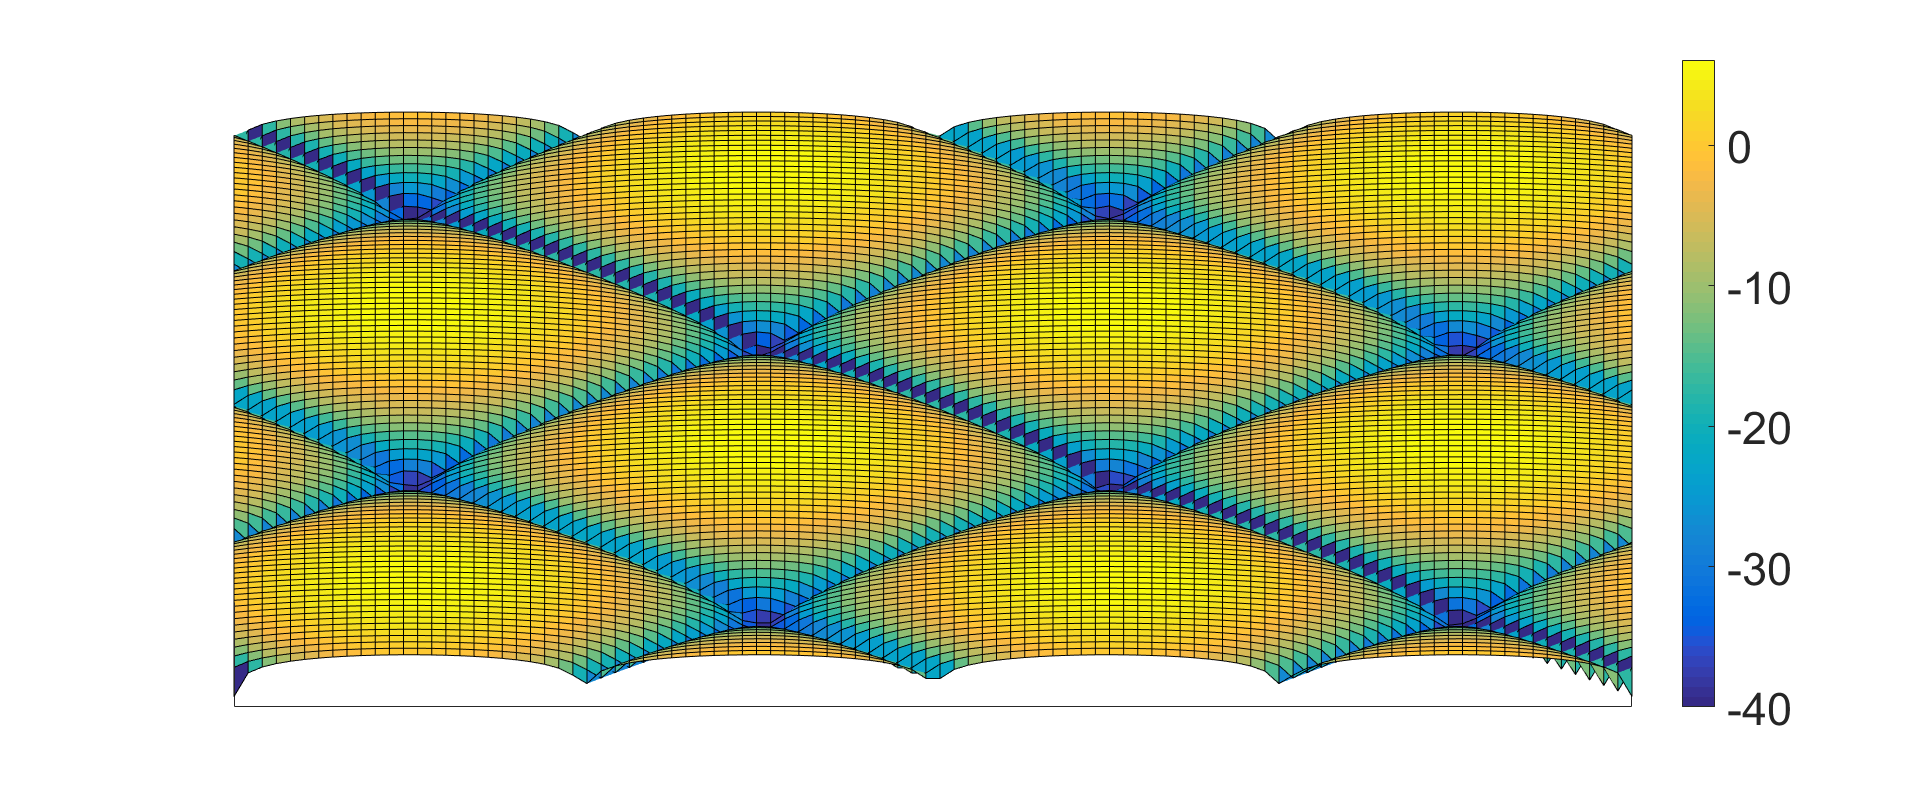
\includegraphics[width=\textwidth]{figures/intro_fading.png}
\caption{Fading gain from two wave fronts meeting, the deep fade spots have been elevated to allow for a better color resolution.}
\label{intro_fading}
\end{figure}\todo{chance picture}

\section{Motivation}

The fading problem is already addressed in cellular networks like \gls{LTE}, \gls{LTE-A} etc. The upcoming 5G network will have new concepts it is proposed to consist of three parts: \Gls{URLLC}, \gls{mMTC} and \gls{eMBB} \citep{5G}. Both the \gls{mMTC} and \gls{eMBB} will be sort of extensions to the existing networks, focusing on either the number of users or the data rate respectively. \Gls{URLLC} will introduce some new problems mostly in the reliability aspect where existing networks operate with an outage probability of 0.1\%, while the URLLC part shall have an outage probability under 0.001-0.0001\% \citep{LTE,Petar5G} and will also lower the latency from (>30 to <1) ms \citep{LTE,5G_Latency}. 

By introducing this new feature, critical system with special needs might be able to use the cellular network instead of a wired channel. A wired channel provides a higher reliability, but comes with a greater cost in both price and installation. It is predicted that some of the applications needing a URLLC channel in the future could be self driving cars, emergency services and sensitive machinery like a remote surgery system \citep{Petar5G}. Common for these examples is that they all require both low latency and low outage probability. Other systems that can gain advantages with URLLC, is systems where the communication window is very small and therefore do not have time for re-transmissions or a lot of data processing for error coding.


The problem is that in the URLLC scenarios, an in depth description of the channel is needed. A way to get higher reliability is to transmit with a higher power level, so the \gls{SNR} gets stronger on the communication link. But even if the overall signal is stronger, there will still be problem with fading in some points in space as seen in \autoref{intro_fading}. Today descriptions of such channels have been verified to a probability level down to around 1E-4. Existing research is assuming that an extrapolation of the Rayleigh model extend to probability levels that are multiple magnitudes lower as seen in \autoref{fading_gain}. This might have been all right so far, but to achieve URLLC conditions the channel needs to be tested at very deep fades down to -50 dB. Therefore this report wants to investigate untested assumptions made in multipath fading channels. The problem when testing such channels is that current measuring systems are not designed for the needed dynamic range or the large amount of samples needed to measure these very deep fades. 

\begin{figure}[H]
\centering
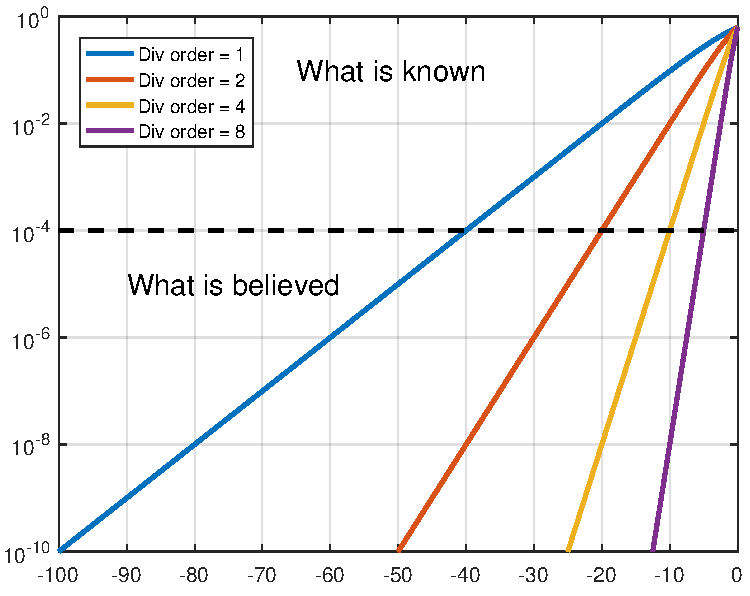
\includegraphics[width=0.65\textwidth]{figures/fading_gain.pdf}
\caption{\Gls{CDF} of Rayleigh fading gain with different diversity orders.}
\label{fading_gain}
\end{figure}


\textbf{Problem statement:}
Design a measurement system that can handle very deep fades and a statistical method to process the data and compare to existing Rayleigh model used in URLLC channels.

%This can be further specified to a more technical problem statement: \todo{Where do these numbers come from and why do we have two statements just after each other?!?}

%Ascertain with 90\% confidence with a 1 dB (25\%) margin that in a multipath environment, the cumulative distribution function of the fading gain can be assumed to increase in a log log linear fashion between -50dB and -20dB.


To achieve this it is important to investigate the following points: 
\begin{itemize}
	\item Find connections between channel statistics and sample size.
	\item Find the reasonable confidence interval based on the minimum required sample size.
	\begin{itemize}
	\item Look into if there is a way to reduce the amount of samples needed by using statistical techniques.
 	\end{itemize}
	\item Figure out how to obtain uncorrelated samples in temporal and spatial domains.
	\item Balance the sample acquisition for available resources. 
	\item Design  a measurement setup that can acquire the samples needed.
	\item Specify a method to process the obtained channel measurements.
	\item Analyse the measurement and link the results to the used assumptions.
\end{itemize}





\section{Project outline}

The focus will be to measure and compare channel characteristics at URLLC conditions. The project will not address the issue of low latency, as this is a completely different issue. The main aspect becomes the wireless channel and its practical limitations focusing on fading. To investigate the channel, a test setup that can measure the varying signal power due to fading is needed. This gives two main aspects for this project as seen on \autoref{ChannelAndEquip}.

\begin{figure}[H]
\centering
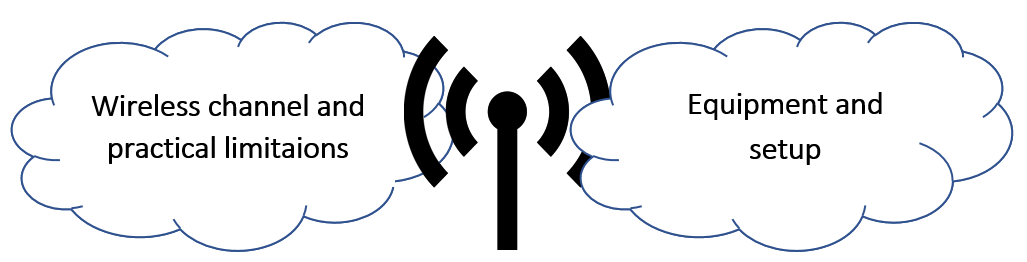
\includegraphics[width=0.85\textwidth]{figures/ProOutline.png}
\caption{The two main aspects of the project.}
\label{ChannelAndEquip}
\end{figure}



The rest of the report is structured as follows. In part I the general and theoretical problems are investigated. Chapter 2 of the report will explain some basic statistics in relation to brute force estimation. When a number of samples required is established, statistical techniques is explored to see if it is possible to reduce the amount of samples needed. In Chapter 3 the wireless channel is discussed in general together with  the ideas of multipath and fading channels. This will give a method to obtain uncorrelated samples in wireless channels. Chapter 4 goes through a basic receiver structure to examine potential problems and requirements of the measurements. By establishing these principals of the wireless channels and multipath fading the measurement setup is designed in part II. Chapter 5 describe the available resources for the measurements followed by chapter 6 that goes through the general setup parameters used for during measurements. Chapter 7 and 8 discusses the coherence bandwidth test and the fading measurements respectively. The results are extensively analysed and presented together with the Rayleigh fading model. Next is the discussion of uncertainties in the measurement campaign in chapter 9 and finally the conclusion in chapter 10.

%First some values from previous scientific research and theory is used to estimate  parameters needed in the measurement. This gives a insight in our thought process when designing the measurement setup how do address  our limitations. The final settings and values used in the measurement is given together with the raw results. The following part is the analysis and presentation of the findings from the measurement. After that, the next chapter includes the  discussion of the uncertainties and difficulties that occurred. The final chapter contains the conclusions of the report.




 




